\documentclass[a4paper,utf8]{article}
\usepackage{rapport}
\usepackage[normalem]{ulem}
\usepackage{amsfonts}
\usepackage{graphicx}
\usepackage{MnSymbol,wasysym}
\usepackage{hyperref}
\usepackage[french]{babel}


\formation{L3MI}
\date{}
\matiere{Conception Orient�e Objet}
\titre{Dots And Boxes - Compte Rendu}

\newcommand\code[1]{\textsf{#1}}
\newcommand\srdjan[1]{{\color{red} #1}}

\begin{document}

\entete

\section{Ce qui a �t� r�alis�}

-Impl�mentation du jeu en MVC (Quelques confusions sur le menu)\\%
-Impl�mentation d\textquotesingle une IA \\%
-Menu de gestion du nombre de joueurs, du type de joueurs (Humain/IA), du nombre de cases. \\%

\section{Ce qui a �t� r�alis�}

Pour r�pondre au probl�me, on va mod�liser la grille de la mani�re suivante : \\%
-Un ensemble de traits verticaux \\%
-Un ensemble de traits horizontaux \\%
-Un ensemble de cases \\%
\\%
Chaque attribut dispose d\textquotesingle une valeur associ� � un joueur.\\%
A l\textquotesingle initialisation, aucun attribut n\textquotesingle est assign� aux joueurs.\\%

\makebox[\textwidth]{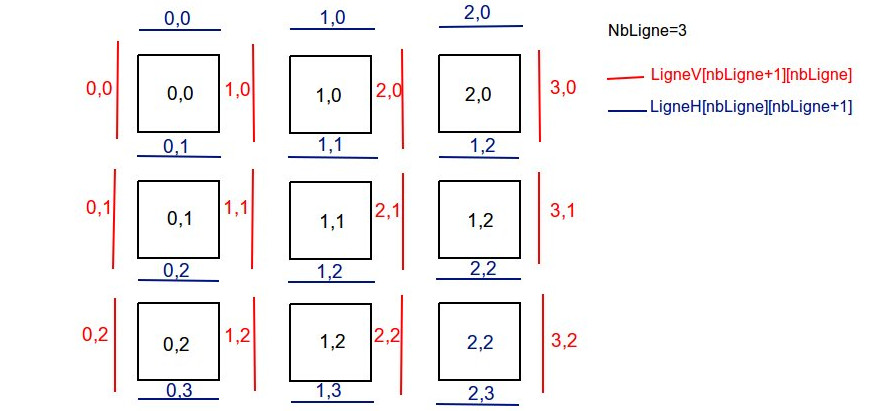
\includegraphics[width=500pt]{img/image12}}


\section{M�thode de d�cision de l\textquotesingle IA}

\subsection{Mod�lisation} 

Premi�re chose � dire, chaque trait a une influence sur au plus 2 carr�s. (1 seul pour les bordures).\\%
\\%
Pour chaque trait, on va regarder les carr�s auxquels il appartient.\\%
Apr�s avoir r�cup�r� le(s) carr�(s), on va compter les cot�s appartenant � un joueur, et on va �tablir un couple de 2 entiers. (-1 si pas de carr�s possibles )\\%

Exemple : \\%
TraitH (3,4) si on ajoute le trait, on aura 3 traits/4 sur le carr� du haut, et un carr� entier sur le carr� du dessous.\\%
TraitV (-1,2) Trait sur la bordure gauche, on aura 2 traits/4 sur le carr� de droite.\\%
\\%


\subsection{D�cision} 

L\textquotesingle IA va alors choisir de mani�re al�atoire et dans l\textquotesingle ordre de priorit� suivant le couple le plus adapt� :\\%
\\%
+++\\%
\^\\%
\textbar (4,4) : Optimal, On peut former deux carr�s  \\%
\textbar (4,1)/(1,4) : Prioritaire (forme un carr� et aucun avantage pour l\textquotesingle autre joueur)\\%
\textbar (4,2)/(2,4) : Prioritaire (forme un carr� et aucun avantage pour l\textquotesingle autre joueur)\\%
\textbar (4,3)/(3,4) : (Forme un carr� mais avantage pour l\textquotesingle autre joueur)\\%
\textbar (1,1) : Aucun risque\\%
\textbar ...\\%
\textbar ...\\%
\textbar (3,1)/(1,3) : Laisse un carr� pour l\textquotesingle autre joueur\\%
\textbar (3,2)/(2,3) : Laisse un carr� pour l\textquotesingle autre joueur\\%
\textbar (3,3)/(3,3) : Pire cas, 2 carr� pour l\textquotesingle autre joueur\\%
- - -\\%

\makebox[\textwidth]{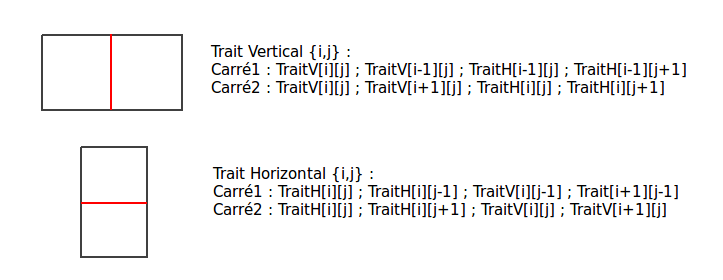
\includegraphics[width=400pt]{img/image2}}


\end{document}